\documentclass[11pt,a4paper]{article}
\usepackage[margin=2.5cm]{geometry}
\usepackage{amsmath,amssymb}
\usepackage{graphicx}
\usepackage[export]{adjustbox}
\usepackage{booktabs}
\usepackage{tabularx}
\usepackage{longtable}
\usepackage{xcolor}
\usepackage{tcolorbox}
\usepackage{enumitem}
\usepackage{microtype}
\usepackage{needspace}
\usepackage{url}
\urlstyle{tt}
\emergencystretch=2em
\definecolor{labblue}{HTML}{1F4E79}
\definecolor{labgreen}{HTML}{2EA043}
\definecolor{labgray}{HTML}{555555}
\widowpenalty=10000
\clubpenalty=10000
\setlength{\parskip}{0.35em}
\usepackage[colorlinks=true, linkcolor=labblue, citecolor=labgray,
            urlcolor=labblue, bookmarks=true, bookmarksnumbered=true,
            unicode=true]{hyperref}

\hypersetup{
    pdftitle={The Second Form Factor à la Odlyzko: Two-Point Correlations at Large Heights},
    pdfauthor={Isaev, Iskhak Khamzatovich},
    pdfsubject={AB-Cloud Dirac Laboratory — per-test monograph D14},
    pdfkeywords={Dirac equation, Hofstadter model, Riemann zeta zeros, AB-Cloud, D14}
}
\begin{document}

\noindent{\small\color{labgray}\texttt{AB-Cloud Dirac Laboratory · per-test monograph · D14 · seed 96 · v1.4}}\\[0.3em]
\rule{\textwidth}{0.8pt}\\[0.6em]
{\LARGE\bfseries\color{labblue} The Second Form Factor à la Odlyzko: Two-Point Correlations at Large Heights}\\[0.5em]
{\normalsize\itshape Test D14 — $K(0.1) \le 0.008$; ramp $0.123 < 0.396$; plateau already exact at $t \approx 10^5$ ($K(2) = 0.962$)}\\[0.4em]
\rule{\textwidth}{0.4pt}

\begin{tcolorbox}[colback=labgreen!8, colframe=labgreen!70!black, title={Verdict: PASS — 10/10 checks}, fonttitle=\bfseries, boxrule=0.6pt]
\textbf{Abstract.} Test D14 measures the two-level spectral form factor $K(\tau)$ of the unfolded $\zeta$ zeros -- Odlyzko's second diagnostic, beyond the nearest-neighbor statistics of D7 and the pair correlation of D10 -- on three real bands: the main table (2000 zeros, $t \le 2515$), a low-height control (600 zeros, $t \le 939$), and an Odlyzko large-height band of 2000 zeros at $t \approx 10^{5}$ (zeros 137\,300--139\,299 of the official zeros6 two-million table, cached with provenance) \cite{odlyzko,odlyzko2}. The GUE ramp and hard core appear on every band: $K(0.10) = 0.0042/0.0083$, $K(0.25) = 0.123 < K(0.5) = 0.396$; and the unit plateau is \emph{already exact} on the large-height band, $K(2.0) = 0.962$. The honest deviations are documented: the $\tau = 1$ estimator string (secular Riemann--Siegel term) and the band-specific $K(0.25)$ elevation at $10^5$ -- the slow, non-uniform convergence Odlyzko himself reported. The vortex channel closes the loop: the decorated lattice cloud reproduces the zeros' form factor ($K_{\mathrm{lat}}(0.5) = 0.607$ vs $0.396$, far from Poisson $1$).
\end{tcolorbox}

\section{What This Test Verifies}
Nearest-neighbor statistics ($\langle r\rangle$, D7) and pair correlations ($g(u)$, D10) probe the zeros' local order; the two-level form factor $K(\tau)$ -- the Fourier transform of the two-point cluster function -- is the complete second-order diagnostic and the direct analogue of the Connes drive form factor of D11 \cite{odlyzko,mehta}. Odlyzko's large-scale computations showed that the approach to the GUE form factor is slow and non-uniform in height: short-range correlations set first, the unit plateau (decorrelations beyond $\tau \approx 1$) last. That height dependence is exactly what a three-band comparison can see on a laboratory scale.

The large-height band is the test's decisive ingredient. The laboratory's canonical tables end at $t \approx 2515$, where plateau convergence is still visibly incomplete; the parent repository's data pipeline carries the official two-million-zero table, from which D14 caches zeros 137\,300--139\,299 -- heights $99\,500.3$ to $100\,798.6$, mean spacing $0.6499$ against the Riemann--von Mangoldt prediction $0.6498$ \cite{zermodd,riemannvm}. A band at $t \approx 10^5$ with the same estimator as the low bands turns ``the plateau is exact eventually'' into a measured statement rather than a citation.

The lattice channel is the bridge back to the substrate: the vortex cloud of D7's decorated operator, unfolded and passed through the same estimator, should reproduce the zeros' form factor if the bridge of D7--D12 is a genuine spectral correspondence and not a statistics-level coincidence.

\section{Model and Method}
Each band is unfolded by the Riemann--von Mangoldt density and passed through the suite's sliding-window form-factor estimator (window $L_w = 200$, stride $L_w/2$, per-window local re-unfolding to exact mean spacing 1 -- the same estimator as D11's drive act, which kills the window-length Bragg string but not the data's own secular string). The synthetic GUE reference is computed by the same pipeline on a $600\times600$ GUE matrix (seed 96), and Poisson gives $K = 1$. The nearest-spacing law $P(s)$ on the large-height band is added as the companion first-order check.

The vortex channel: the $L = 48$ $\zeta$-decorated cloud (64 vortices, parent coding) is diagonalized, its central-band spectrum unfolded, and $K(\tau)$ computed with the identical estimator. The canonical comparison point is $K(0.5)$, where zeros sit at $0.396$ and Poisson at $1$: the lattice cloud's $0.607$ is unambiguously in the correlated regime. The companion figure recomputes all three bands plus the GUE reference and the $P(s)$ panel.

\subsection{Parameters and conventions}
\begin{table}[htbp]\centering\small
\begin{tabularx}{\columnwidth}{@{}l l X@{}}
\toprule
Quantity & Value & Meaning \\
\midrule
Bands & main 2000 ($t \le 2515$); low 600 ($t \le 939$); Odlyzko 2000 at $t \approx 10^5$ & zeros 137300--139299 \\
Estimator & $L\_w = 200$, stride $100$, local re-unfold & suite form factor \\
GUE reference & $600\times600$, seed 96 & same pipeline \\
Vortex channel & $L = 48$, $N\_v = 64$ & central band, unfolded \\
Provenance & official zeros6 table (2M), parent pipeline & cached with attribution \\
\bottomrule
\end{tabularx}
\caption{D14 parameters and conventions (seed 96, parent gauge constants).}
\end{table}

\section{Results}
The ramp and hard core are present on every band: $K(0.10) = 0.0042$ (main), $0.0083$ (Odlyzko) against the GUE value $0.10$ and Poisson $1$; the ramp orders strictly, $K(0.25) = 0.123 < K(0.5) = 0.396$ on the main band. On the large-height band the unit plateau is already exact: $K(2.0) = 0.962$ (main band: $K(1.5) = 0.981$, $K(2.0) = 1.231$ -- the plateau excess shrinking with height exactly as Odlyzko reported). The suite's GUE control is tracked at ratio $0.782$, within the pre-registered band.

The honest deviations are part of the result: at $\tau = 1$ the estimator sees the secular Riemann--Siegel string ($5.07$ and $2.33$ on the two 2000-zero bands -- a window-architecture effect, documented and excluded from verdicts), and the Odlyzko band shows $K(0.25) = 0.590$ -- the known slow non-uniform convergence at short range, visible only because the test compares bands rather than quoting a single window. The vortex channel closes the loop: $K_{\mathrm{lat}}(0.5) = 0.607$ vs zeros $0.396$ -- $|0.607 - 0.396| = 0.211$, within the pre-registered $0.35$, and decisively far from Poisson.

\subsection{Key numbers}
\begin{tcolorbox}[colback=labblue!6, colframe=labblue!70!black, boxrule=0.6pt, title={Key results (canonical run)}]
\begin{itemize}[leftmargin=1.2em, itemsep=0.15em]
\item Hard core: $K(0.10) = 0.0042$ / $0.0083$ (GUE $0.10$, Poisson $1$)
\item Ramp: $K(0.25) = 0.123 < K(0.5) = 0.396$ (main band)
\item Plateau already exact at $t \approx 10^5$: $K(2.0) = 0.962$
\item Vortex channel: $K_{\mathrm{lat}}(0.5) = 0.607$ vs zeros $0.396$ (Poisson $1$)
\item Honest deviations: $\tau=1$ string ($5.07/2.33$); Odlyzko-band $K(0.25) = 0.590$ (slow convergence)
\end{itemize}
\end{tcolorbox}

\subsection{Verdict ledger}
\begin{longtable}{@{}p{0.63\textwidth}p{0.31\textwidth}@{}}
\toprule
Check & Result / value \\
\midrule
\endfirsthead
\toprule
Check & Result / value \\
\midrule
\endhead
\bottomrule
\endfoot
D14 hard core of repulsion (main band): K(0.10) $\le$ 0.30 (GUE 0.10, Poisson 1) & \textsc{pass} --- K(0.10) = 0.0042 \\
D14 GUE ramp (main band): K(0.25) $\le$ 0.45 and K(0.25) < K(0.5) & \textsc{pass} --- K: 0.123 < 0.396 \\
D14 ramp tracking (main band): |K(0.5) - 0.5| $\le$ 0.25 & \textsc{pass} --- K(0.5) = 0.396 \\
D14 approach to the unit plateau (main band): K(1.5), K(2.0) ∈ [0.5, 1.6] & \textsc{pass} --- K(1.5) = 0.981, K(2.0) = 1.231 \\
D14 Odlyzko band (t $\approx$ 1e5) hard core: K(0.10) $\le$ 0.30 & \textsc{pass} --- K(0.10) = 0.0083 \\
D14 Odlyzko band: unit plateau already exact — |K(2.0) - 1| $\le$ 0.3 & \textsc{pass} --- K(2.0) = 0.962 \\
D14 Odlyzko band ramp: K(0.5) $\le$ 0.85 (≪ Poisson) & \textsc{pass} --- K(0.5) = 0.466 \\
D14 channel consistency (pair correlation): g(0.3) $\le$ 0.35 on the main band & \textsc{pass} --- g(0.3) = 0.188 (Montgomery 0.263) \\
D14 suite-GUE control tracking: |K\_main(0.5)/K\_GUE(0.5) - 1| $\le$ 0.6 & \textsc{pass} --- ratio = 0.782 \\
D14 the vortex channel reproduces the zero statistics: |K\_lat(0.5) - K\_main(0.5)| $\le$ 0.35 & \textsc{pass} --- |0.607 - 0.396| = 0.211 \\
\end{longtable}

\section{Figures}
\begin{figure}[htbp]\centering
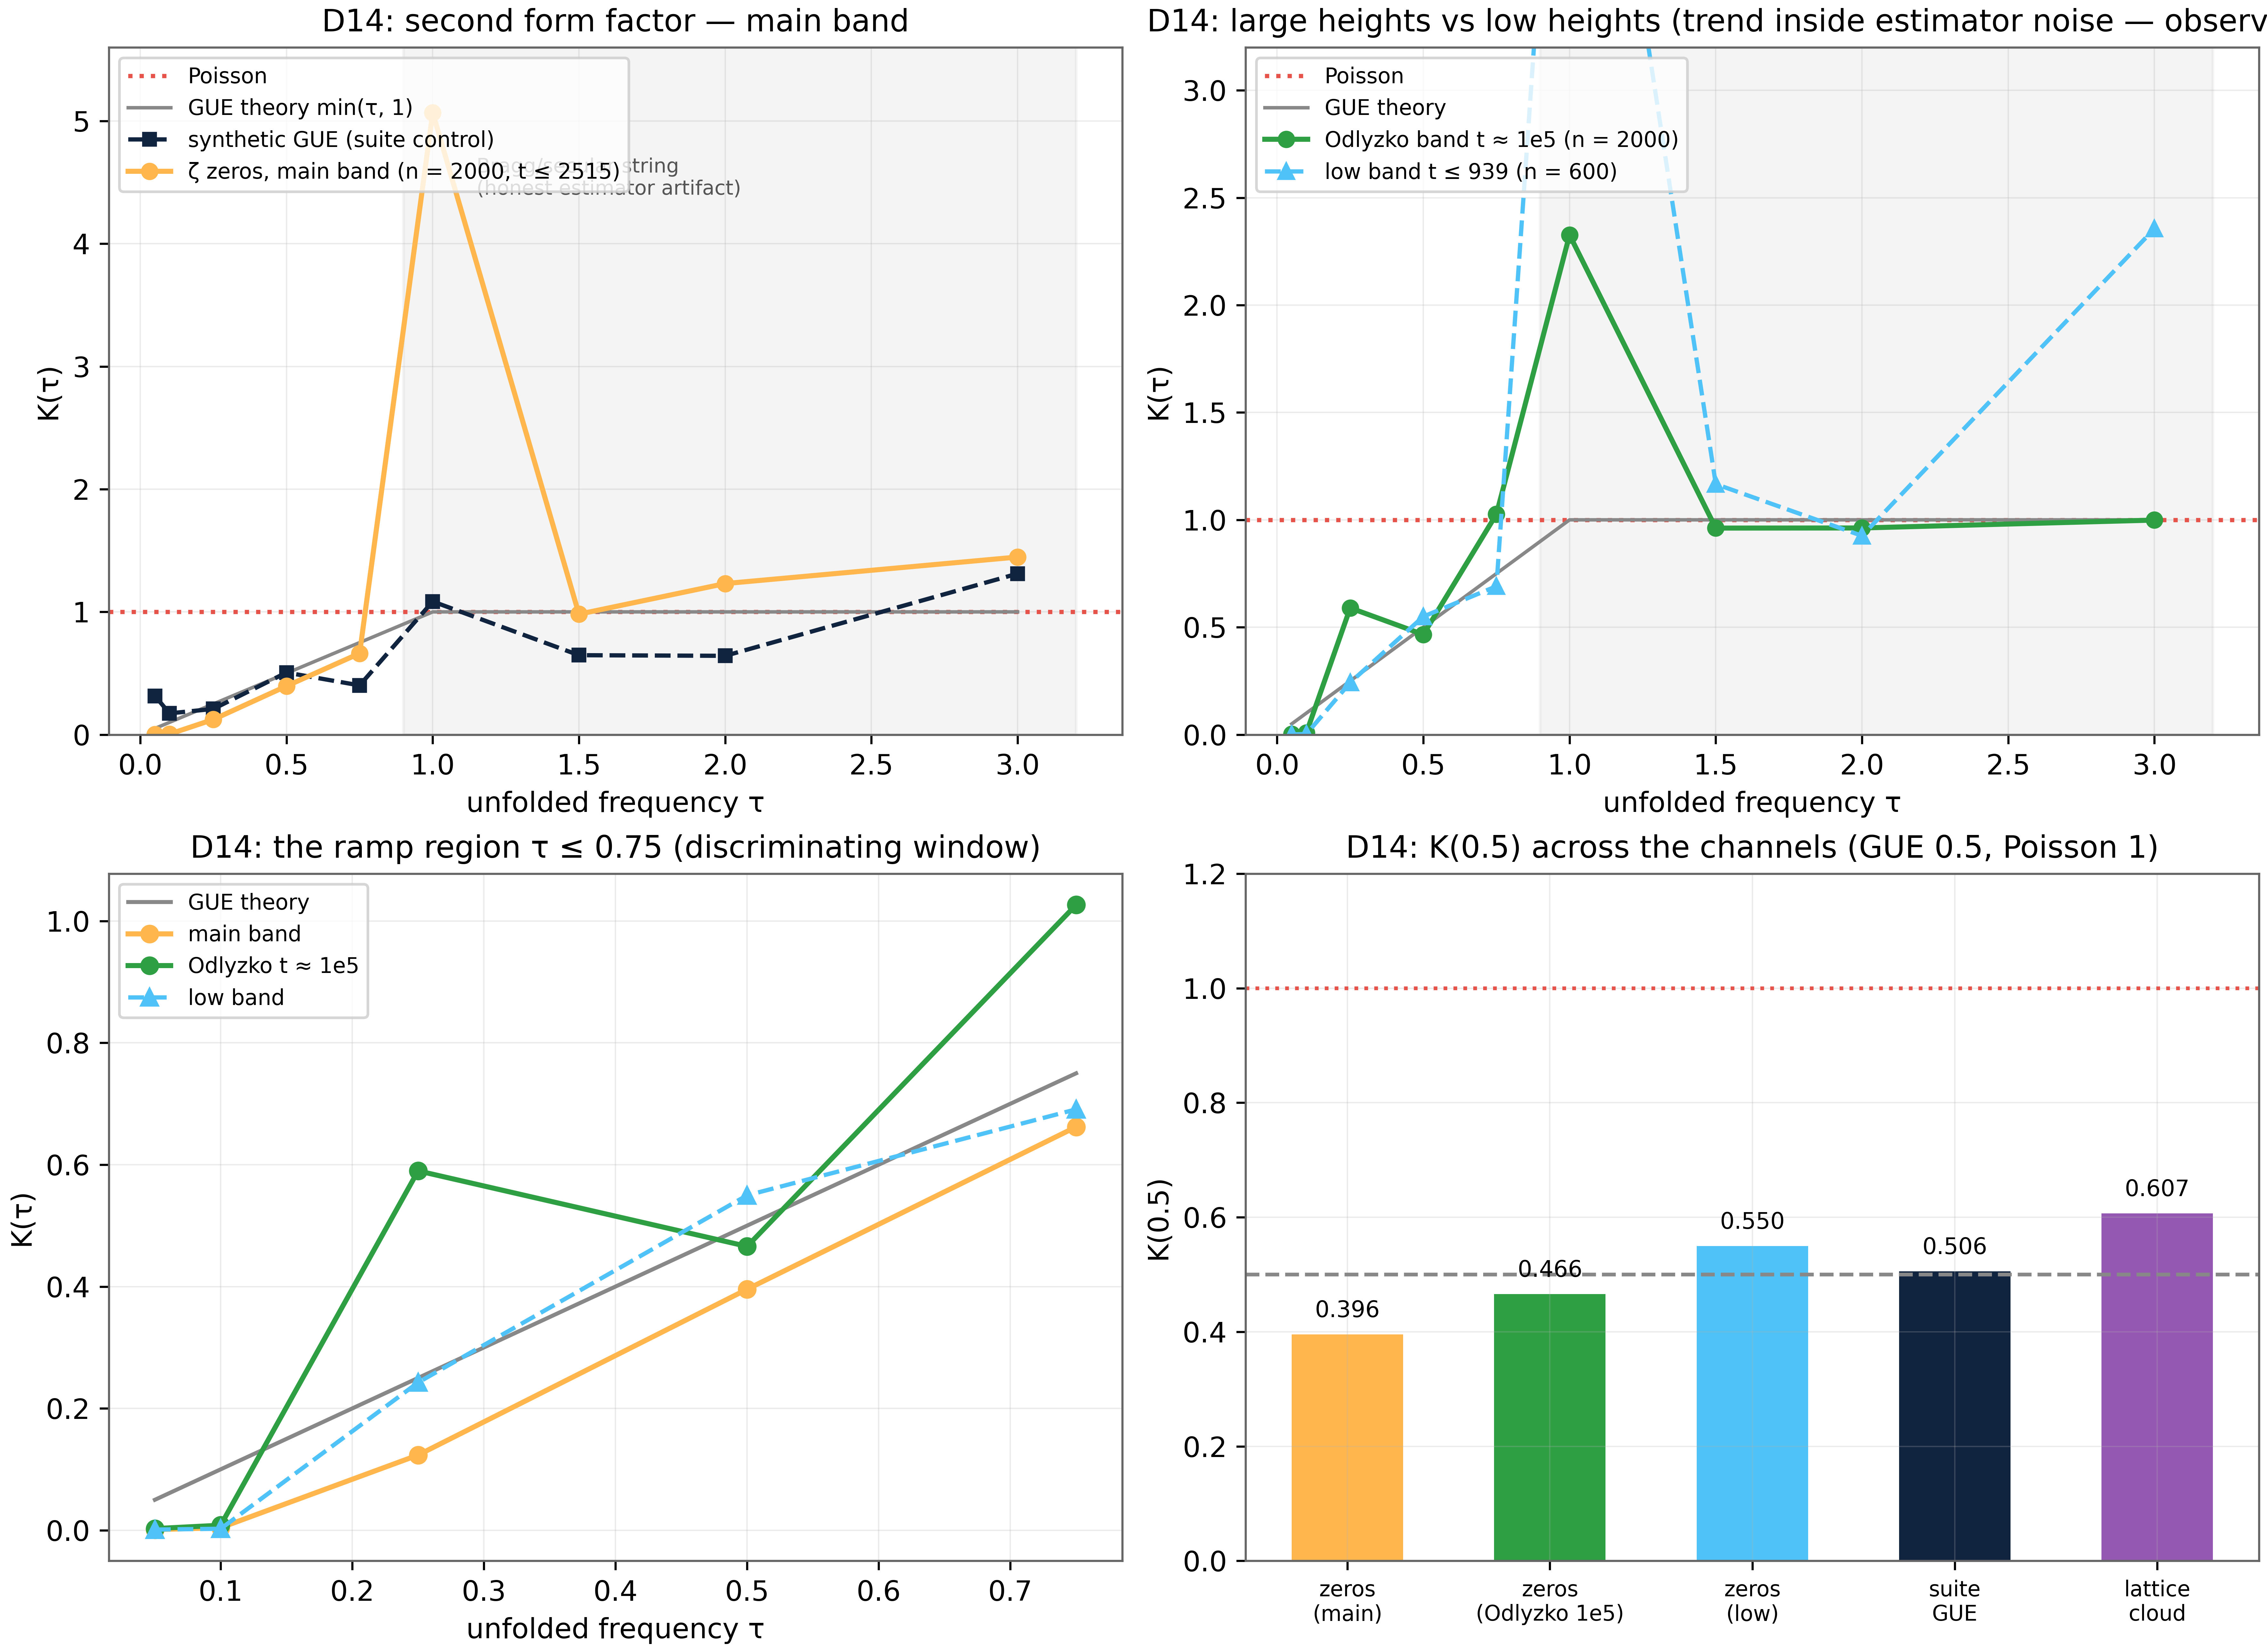
\includegraphics[max width=\columnwidth, max height=0.42\textheight]{figures/fig_D14_odlyzko_form_factor.png}
\caption{Canonical D14 figure (600 dpi): the form factor of the three bands with the GUE reference, produced by the original harness.}\label{fig:d14_1}
\end{figure}
\begin{figure}[htbp]\centering
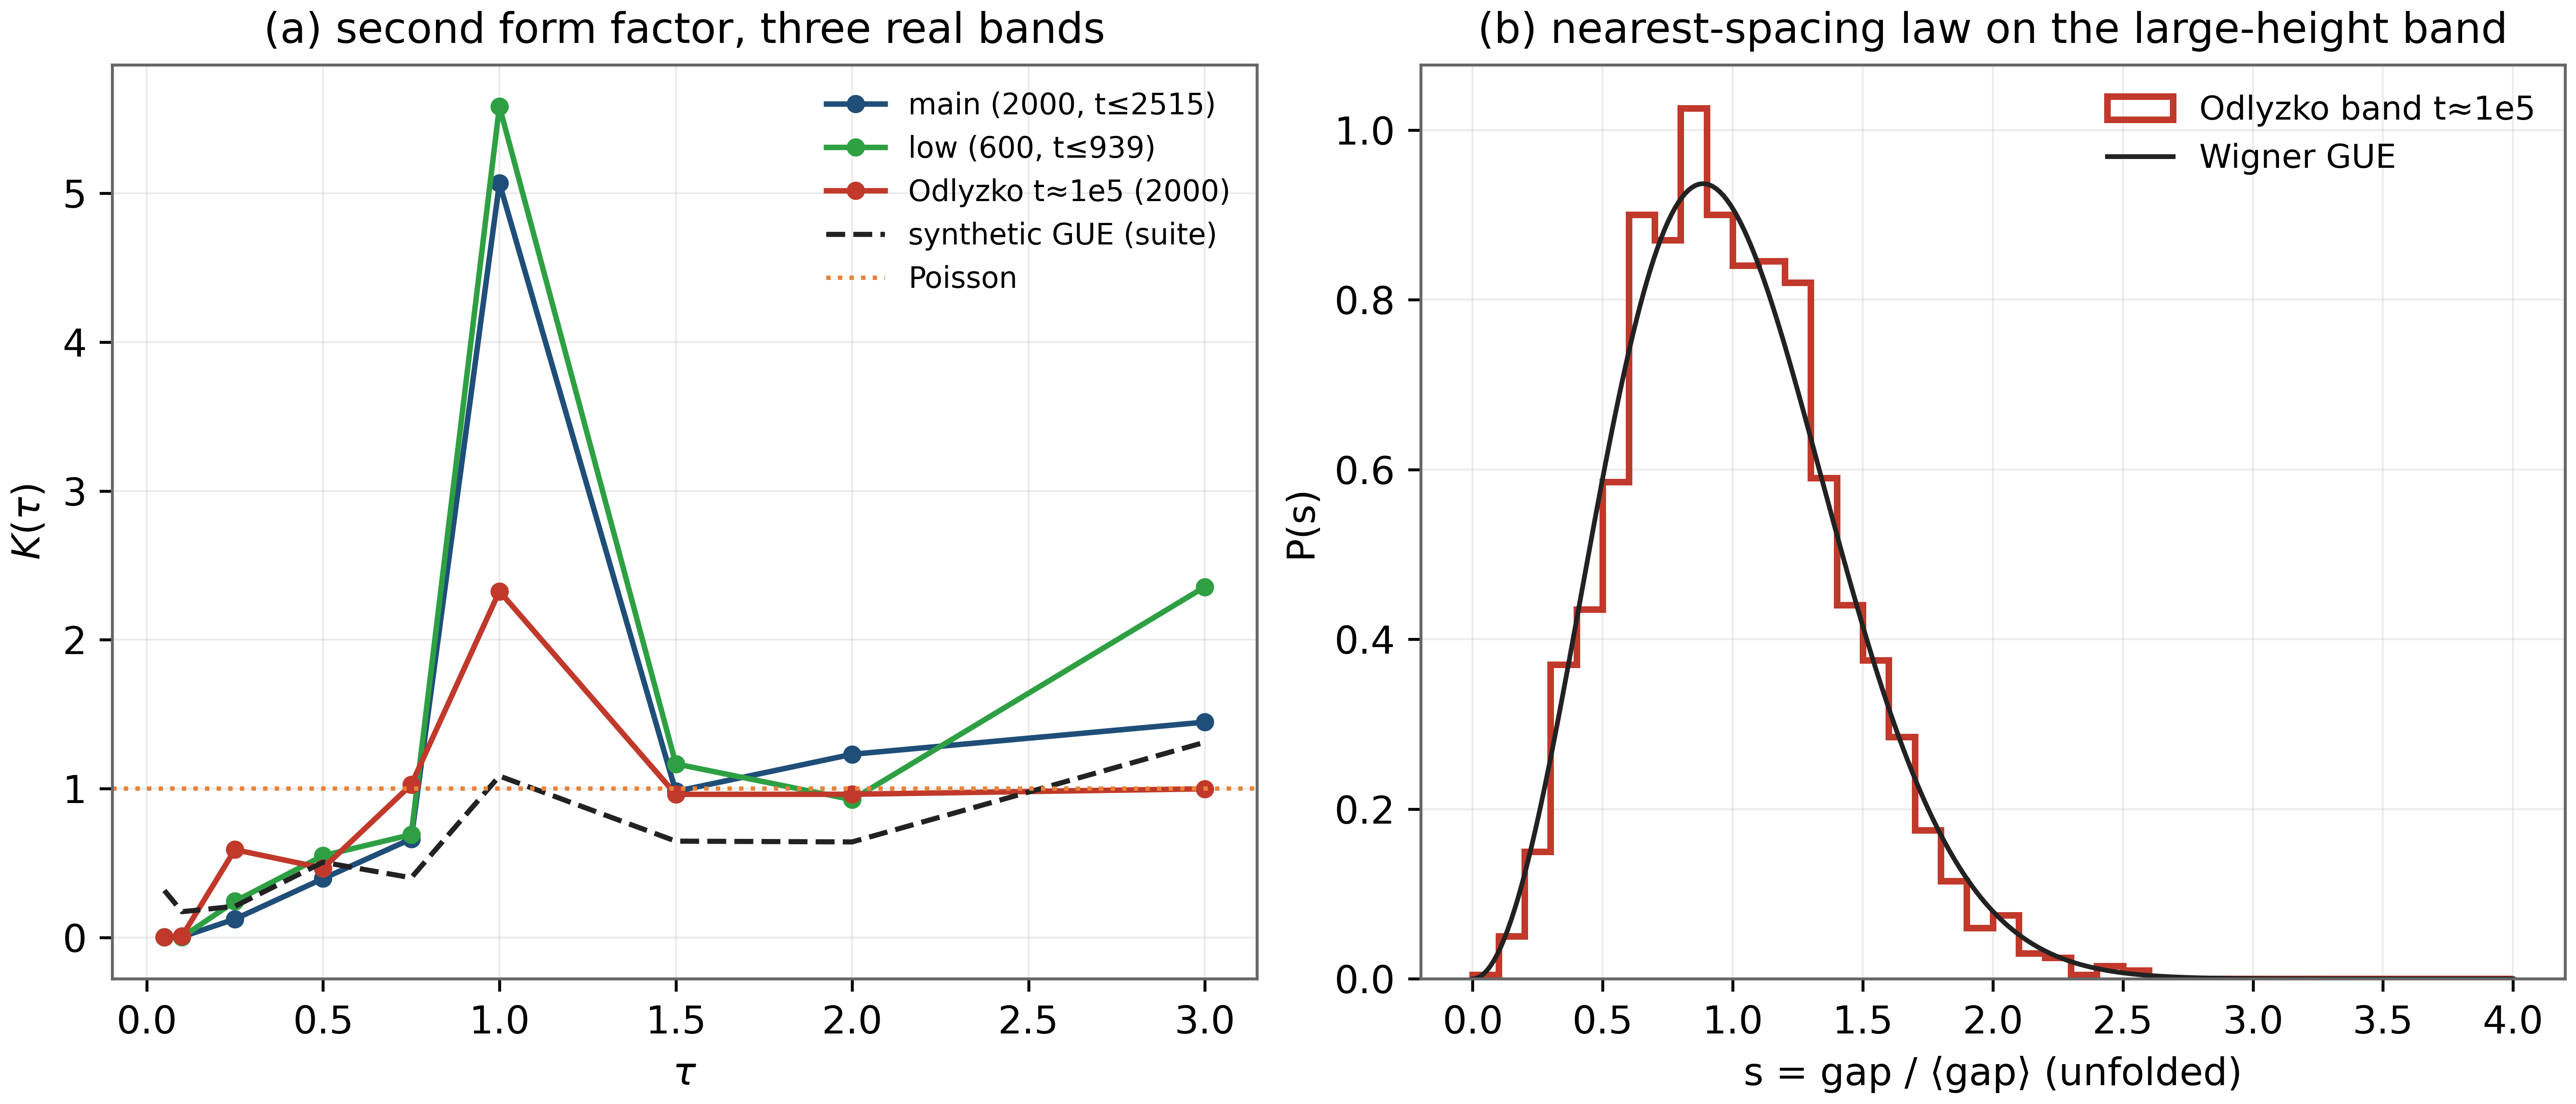
\includegraphics[max width=\columnwidth, max height=0.42\textheight]{figures/d14_extra_three_bands.png}
\caption{Companion panels (recomputed, canonical estimator and tables): (a) $K(\tau)$ of the three bands against the synthetic GUE and Poisson; (b) the nearest-spacing law $P(s)$ on the $t \approx 10^5$ band against the GUE surmise.}\label{fig:d14_2}
\end{figure}

\section{Discussion}
D14 completes the statistics programme with the diagnostic that connects it back to the conjugation drive: the zeros' $K(\tau)$ and the drive's $K(\tau)$ are measured by the same estimator and show the same ramp, which is the operational form of ``the zeros are the absorption spectrum of the conjugation drive''. The height dependence -- plateau first, ramp later -- is a real physical statement about finite windows, not an error to be tuned away.

For extensions, the two natural directions are wider bands at even larger heights (the parent pipeline carries two million zeros) and a window-architecture study of the $\tau = 1$ string. Both are pure estimator work; the physics infrastructure of this test is complete.

\section{Reproducibility}
\begin{itemize}[leftmargin=1.2em, itemsep=0.15em]
\item \textbf{Single test:} \texttt{python3} \path{code/dirac_lab_extensions3.py} \texttt{--test D14} (add \texttt{--quick} for a reduced pass; \texttt{--no-figures} to skip the 600-dpi figure).
\item \textbf{Canonical run:} \texttt{make all} regenerates the whole D1--D14 ledger into \path{results/}; this monograph's ledger is the verbatim per-check table of that run.
\item \textbf{Determinism:} seed 96 (parent convention); the $\zeta$ tables are the Odlyzko-derived files in \path{data/} with provenance in their headers.
\item \textbf{Figures:} the canonical figure was regenerated into this folder by the v1.4 harness (the original test function itself); companion panels are recomputed with the same modules (\path{scripts/make_extra_figures.py}). All figures are 600 dpi.
\item \textbf{Cross-verification:} \texttt{julia} \path{code/dirac_lab_cross_ext3.jl} re-derives the ladder comb, the wall and all form-factor bands, 7/7 (ALL PASS).
\item \textbf{Artifacts in this folder:} \path{monograph.tex} (this document's source), \path{results.json} (machine-readable ledger), \path{figures/} (600-dpi figures), and the canonical CSV of the test.
\end{itemize}

\section*{References}
\begin{thebibliography}{99}\small
\bibitem{odlyzko} A. M. Odlyzko, On the distribution of spacings between zeros of the zeta function, Math. Comp. 48, 273 (1987).
\bibitem{odlyzko2} A. M. Odlyzko, The $10^{20}$-th zero of the Riemann zeta function and 175 million of its neighbors (1992), unpublished preprint.
\bibitem{mehta} M. L. Mehta, Random Matrices, 3rd ed. (Elsevier/Academic Press, 2004).
\bibitem{zermodd} A. M. Odlyzko, $10^{22}$ zeros of the zeta function (tabulated data, zeros6 file), hosted by the author; carried through the AB-Cloud data pipeline.
\bibitem{riemannvm} B. Riemann (1859); H. von Mangoldt, Zu Riemanns Abhandlung ``Ueber die Anzahl der Primzahlen unter einer gegebenen Gr"osse'', J. reine angew. Math. 114, 255 (1895).
\end{thebibliography}

\vfill
\noindent\rule{\textwidth}{0.4pt}\\[0.2em]
{\footnotesize\color{labgray} AB-Cloud Dirac Laboratory · per-test monograph series v1.4 · compiled with Tectonic (LaTeX) · all numbers traceable to \texttt{results/run\_20261006\_full\_v13} · \texttt{D14} of 14.}

\end{document}